\documentclass[9pt]{beamer}\usepackage[]{graphicx}\usepackage[]{color}
%% maxwidth is the original width if it is less than linewidth
%% otherwise use linewidth (to make sure the graphics do not exceed the margin)
\makeatletter
\def\maxwidth{ %
  \ifdim\Gin@nat@width>\linewidth
    \linewidth
  \else
    \Gin@nat@width
  \fi
}
\makeatother

\definecolor{fgcolor}{rgb}{0.345, 0.345, 0.345}
\newcommand{\hlnum}[1]{\textcolor[rgb]{0.686,0.059,0.569}{#1}}%
\newcommand{\hlstr}[1]{\textcolor[rgb]{0.192,0.494,0.8}{#1}}%
\newcommand{\hlcom}[1]{\textcolor[rgb]{0.678,0.584,0.686}{\textit{#1}}}%
\newcommand{\hlopt}[1]{\textcolor[rgb]{0,0,0}{#1}}%
\newcommand{\hlstd}[1]{\textcolor[rgb]{0.345,0.345,0.345}{#1}}%
\newcommand{\hlkwa}[1]{\textcolor[rgb]{0.161,0.373,0.58}{\textbf{#1}}}%
\newcommand{\hlkwb}[1]{\textcolor[rgb]{0.69,0.353,0.396}{#1}}%
\newcommand{\hlkwc}[1]{\textcolor[rgb]{0.333,0.667,0.333}{#1}}%
\newcommand{\hlkwd}[1]{\textcolor[rgb]{0.737,0.353,0.396}{\textbf{#1}}}%
\let\hlipl\hlkwb

\usepackage{framed}
\makeatletter
\newenvironment{kframe}{%
 \def\at@end@of@kframe{}%
 \ifinner\ifhmode%
  \def\at@end@of@kframe{\end{minipage}}%
  \begin{minipage}{\columnwidth}%
 \fi\fi%
 \def\FrameCommand##1{\hskip\@totalleftmargin \hskip-\fboxsep
 \colorbox{shadecolor}{##1}\hskip-\fboxsep
     % There is no \\@totalrightmargin, so:
     \hskip-\linewidth \hskip-\@totalleftmargin \hskip\columnwidth}%
 \MakeFramed {\advance\hsize-\width
   \@totalleftmargin\z@ \linewidth\hsize
   \@setminipage}}%
 {\par\unskip\endMakeFramed%
 \at@end@of@kframe}
\makeatother

\definecolor{shadecolor}{rgb}{.97, .97, .97}
\definecolor{messagecolor}{rgb}{0, 0, 0}
\definecolor{warningcolor}{rgb}{1, 0, 1}
\definecolor{errorcolor}{rgb}{1, 0, 0}
\newenvironment{knitrout}{}{} % an empty environment to be redefined in TeX

\usepackage{alltt}

\usepackage{framed}
\usepackage{alltt}
\usepackage{amsmath}
\usepackage{mathtools}
\usepackage{graphicx, color}
\usepackage{natbib}
\usepackage{hyperref}
\usepackage{mathptmx}
\usepackage{beamerthemesplit}
\usepackage{lipsum}

\graphicspath{{../report/figs/}}

\setbeamersize{text margin left=5pt,text margin right=5pt}
\parskip 3mm

\definecolor{firebrick}{RGB}{178,34,34}
\useinnertheme{circles,rounded}
\usecolortheme[named=firebrick]{structure}
\useoutertheme{smoothtree}
\setbeamertemplate{footline}[frame number]

\title{Bayesian inference for covariance matrix}
\author[Ignacio Alvarez-Castro]{Ignacio Alvarez}
\institute[IESTA]{IESTA, Universidad de la República, Uruguay}
\date{ISEC 2018}
\IfFileExists{upquote.sty}{\usepackage{upquote}}{}
\begin{document}
 \frame{\titlepage}
 
 \section{Introduction}
\AtBeginSection[] { 
  \begin{frame}[plain]  
    \tableofcontents[currentsection] 
  \end{frame} 
  \addtocounter{framenumber}{-1} 
} 


	\frame{
		\frametitle{Introduction}
Covariance matrix estimation		
\begin{itemize}
\item  Multivariate normal sampling models 
\item random-intercept, random-slope models 
\begin{eqnarray}
\nonumber y_{ij} &=& \beta_{0j} + \beta_{1j} x_{ij} + \beta_{2j}z_{ij} + \epsilon_{ij} \\
\nonumber  \begin{pmatrix} \beta_{0j} \\ \beta_{1j} \\ \beta_{2j} \end{pmatrix} &\sim&  N \left( \begin{pmatrix} \mu_{0} \\ \mu_{1} \\ \mu_{2} \end{pmatrix} , \Sigma \right) , \;\;\; \epsilon_{ij} \sim N(0, \sigma^2) 
%\nonumber \epsilon &\sim& N(0, \sigma^2) 
\end{eqnarray}
\vspace{1cm}
\item We assess impact of alternative priors for $\Sigma$
\begin{itemize}
\item using simulations
\item with a real data set
\end{itemize}
\end{itemize}
}

\begin{frame}
\frametitle{Problems with the conjugate option}
Inverse Wishart distribution is conjugate and usually available in software. 

However,
\begin{itemize}
\item  ``\textit{implies the same amount of prior information about each of the variance parameters in the covariance matrix}'' \citep{bda2003}.  
\item  relation between $\rho_{ij}$ and $\sigma_i$, higher values for the standard deviation $\sigma_i$ are associated with higher correlations, $\rho_{ij}$ close to 1 or -1 \citep{visualize}. 
\end{itemize}
\vspace{.5cm}

Also, we have found in a scenario with small variability,
\begin{itemize}
\item underestimate correlation
\item overestimate standard deviation
\end{itemize}
\end{frame}


\subsection{Motivation example}
\begin{frame}
\frametitle{Bird counts on Superior forests}
 The Natural Resources Research Institute (University of Minnesota Duluth) carry out monitoring program for study regional population trends of forest birds.
            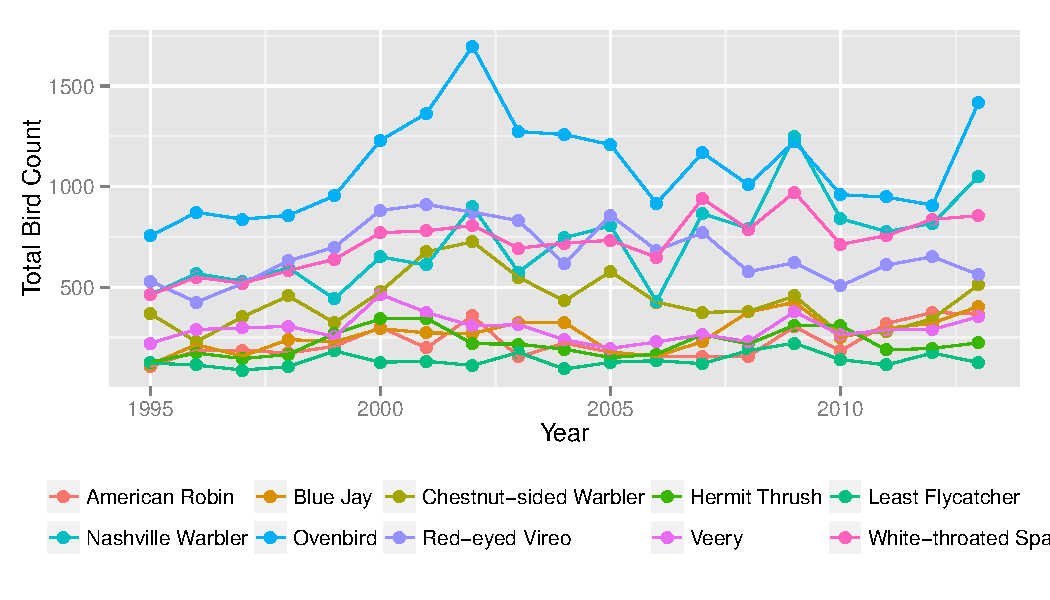
\includegraphics[width=\textwidth, height = 7cm ]{rawtrend}
\end{frame}

\begin{frame}
\frametitle{Quadratic trend model}
  \begin{columns}[T] % the "c" option specifies center vertical alignment
  \column{.5\textwidth} % column designated by a command

\begin{itemize}
  \item $y_{st}$: bird count for spacies $s$ in year $t$.
  \item OLS regression model for each species
\end{itemize}

\[
y_{st}  \sim  N(\beta_{0s} + \beta_{1s} t + \beta_{2t}t^2, \sigma^2)
\]

\vspace{.5cm}

\begin{itemize}
  \item Corr$(\hat\beta_{1s}, \hat\beta_{2s}) = -.77$    
\end{itemize}

  \column{.5\textwidth}
    \includegraphics[scale=.3]{ols_regs}
  \end{columns}

\end{frame}

\begin{frame}
\frametitle{Quadratic trend model}
  \begin{columns}[T] % the "c" option specifies center vertical alignment
  \column{.5\textwidth} % column designated by a command


Use a Bayesian hierarchical linear model with $IW$ prior. 

\[\begin{array}{cl}
y_{st}  & \sim  N(\beta_{0s} + \beta_{1s} t + \beta_{2t}t^2, \sigma^2) \\
& \\
\begin{pmatrix} \beta_{0j} \\ \beta_{1j} \\ \beta_{2j} \end{pmatrix} & \sim  N \left( \begin{pmatrix} 0 \\ 0 \\ 0 \end{pmatrix} , \Sigma \right) \\
& \\
\Sigma & \sim  IW(d+1, I)
\end{array}
\]

Define $\rho = \Sigma_{23}/\sqrt{\Sigma_{22}\Sigma_{33}}$. 

  \column{.5\textwidth}
  \pause
  How does $p(\rho| y)$ look like?
    \includegraphics[scale=.3]{reg_rho_hist}
  \end{columns}
\end{frame}
%============
\section{Covariance matrix priors}

\subsection{Multivariate normal model } 
\begin{frame}
\frametitle{Multivariate normal model }
A simple model: \\
Consider $n$ observations from $Y_i \sim N_d(0, \Sigma)$ distribution. Likelihood function can be written as follows: 
\[
p(y\vert \mu,\Sigma) \propto |\Sigma|^{-n/2} e^{- \frac{1}{2} \sum_{i=1}^n y_i^{'} \Sigma^{-1} y_i  } = |\Sigma|^{-n/2} e^{- \frac{1}{2}  tr(\Sigma^{-1}S_0)  } 
 \]
where $y_i \in R^d$ a realization of $Y_i$,  $S_0=\sum_{i=1}^n y_i y_i ^{'}$, individual entries of $\Sigma$ are $\Sigma_{ii} = \sigma_i^2$ and $\Sigma_{ij} = \sigma_i\sigma_j\rho_{ij}$. 

We compare alternative covariance matrix priors in this context.
\end{frame}

\begin{frame}
\frametitle{ Alternative $\Sigma$ priors}

\begin{description}
\item[$IW(\nu, \Lambda)$] Inverse Wishart:  $\Lambda$ is matrix parameter related to location and $\nu$ degrees of freedom parameter.    \[  p(\Sigma) \propto  |\Sigma|^{-(\nu+ d +1)/2 } e^{-\frac{1}{2} tr( \Lambda \Sigma^{-1}) } \]
\pause

\item[$SIW(\nu, \Lambda, b, \delta)$] Scaled inverse Wishart: $\Sigma = \Delta \; Q \; \Delta$ where $ \Delta_{ii} =\xi_i$, then \[Q \sim IW(\nu, \Lambda) \;\;\;\;\;\;\; \log(\xi_i) \stackrel{ind} \sim N(b_i, \delta_i) \]
\pause

\item[$HIW_{ht}(\nu, \lambda, \delta)$] Hierarchical inverse Wishart:  $\Lambda$ diagonal matrix, $\Lambda_{ii} = \lambda_i$,   \[\Sigma\vert\lambda \sim IW( \nu + d - 1 ,  2\nu\Lambda)  \;\;\;\; \lambda_i \stackrel{ind} \sim \mbox{Ga}\left(\frac{1}{2} , \frac{1}{\delta_i^2}\right) \;\;\; E(\lambda_i)=\frac{\delta_i^2}{2} \]  
\pause

\item[$ BMM_{mu}(\nu, \Lambda, b, \delta)$] Separation strategy: $\Sigma = \Lambda \; R \; \Lambda$  where $\Lambda_{ii}=\sigma_{i}$ and $R=\Delta^q Q \Delta^q$ with $\Delta^q_{ii} = Q_{ii}^{-1/2}$ \[  Q \sim IW(\nu, I )  \;\;\; \log(\sigma_i) \stackrel{ind} \sim N(b_i, \delta_i) \]
\end{description}
\end{frame}

\begin{frame}
\frametitle{ Samples from prior }

\begin{figure}[htbp]
\begin{center}
 \includegraphics[scale=.3]{prior_s1s2_hex} 
%\caption{Scatter-plot of prior samples, relationship among the standard deviation for the first two components (both in log base ten scale). $IW$ prior imply a positive relationship among the standard deviations. Also large correlations values appear the two variance are high and low.} 
\end{center}
\end{figure}

Positive relationship among $\sigma_1$ and $\sigma_2$, also large $|\rho_{12}|$ values appear when the two variances are high.
\end{frame}

\section{Simulation Study}
\begin{frame}
\frametitle{Impact on the posterior inference}

We simulate normally distributed data, 

\[Y \sim N_d(0, \Sigma)\] 

where $d$ represent the dimension, we use $(\Sigma)_{ii} =\sigma \;\; \forall i \in \left\{1,\ldots,d\right\} $ and $(\Sigma)_{ij} = \sigma^2\rho$ which implies all variances and all correlations are equal.

\begin{table}[htbp]
   \caption{Simulation scenarios. Specific values used in simulations for each parameter. \label{scen}} 
   \vspace{-.4cm}
     \begin{tabular}{lcc} \hline
          &  Bivariate    & Ten-dimensional  \\ \hline
      Sample size   ($n$)   & 10,50,250   &  10,50  \\
      Standard deviation ($\sigma$)  & 0.01, 0.1, 1, 10, 100 & 0.01, 1, 100 \\
      Correlation ($\rho$)   &  0, 0,25, 0.5, 0.75, 0.99  &  0, 0.99 \\ \hline
   \end{tabular}
\end{table}
Each scenario is replicated 5 times. 

%We run all models in Stan software, use Potential scale reduction factor for convergence.All models have initially 3 chains with 1000 iterations after burn-in each, initial values disperse on parametric space. 
\end{frame}

\begin{frame}
\frametitle{Inference for $\rho_{12}$}
	\begin{columns}
	 \begin{column}{7cm}
		 \begin{figure}[hbtp]
		   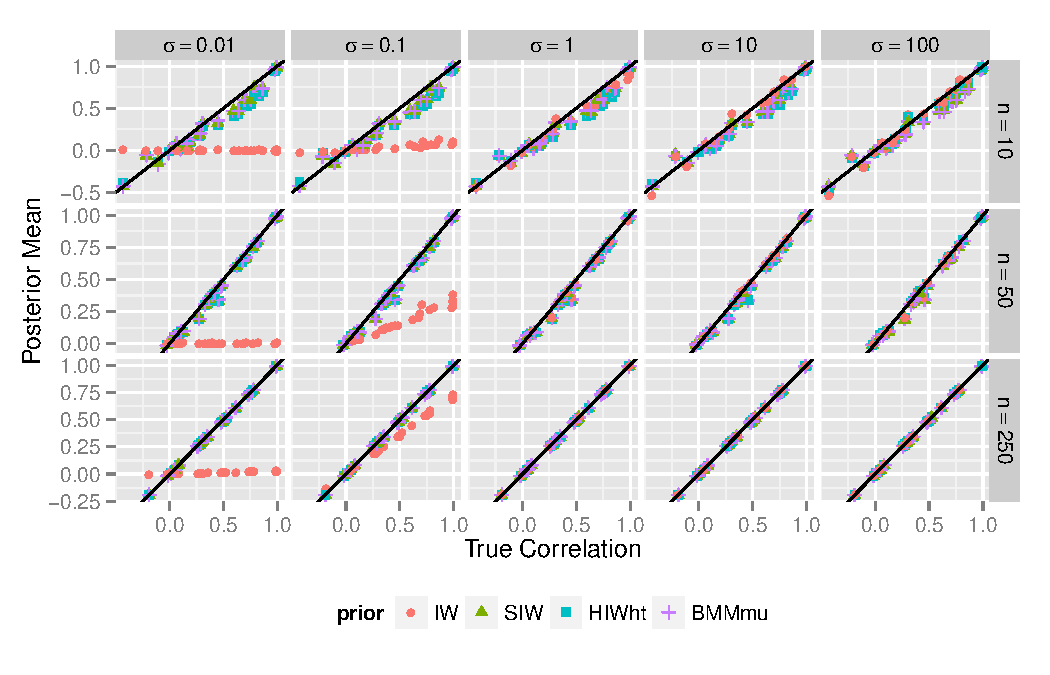
\includegraphics[scale=.4]{fig_rho_d2} 
		\end{figure}
	\end{column}
	\begin{column}{4cm}
	When standard deviation is small, $\sigma=0.01$ or $\sigma=0.1$ the IW prior heavily shrinks the posterior correlation towards 0 even if the true correlation is close to 1. 
	\end{column}
	\end{columns}
\end{frame}

\begin{frame}
\frametitle{Inference for $\sigma_1$}
	\begin{columns}
	 \begin{column}{7cm}
\begin{figure}[htbp]
   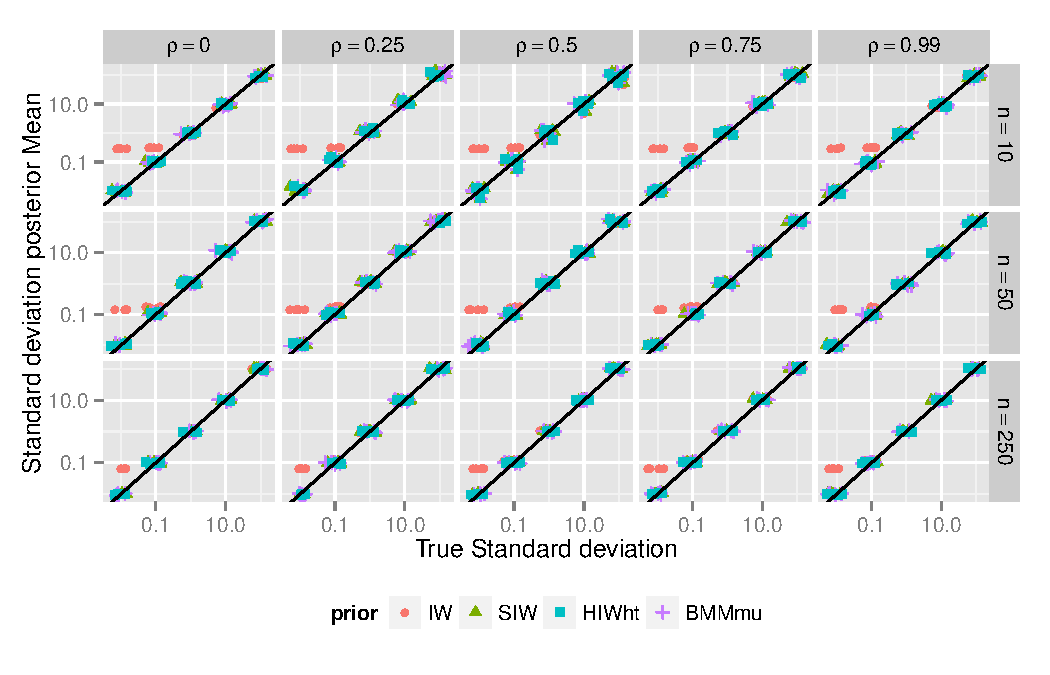
\includegraphics[scale=.4]{fig_s1_d2} 
%   \caption{Scatter-plot of posterior mean for $\sigma_1$  against correlation true standard deviation.}
\end{figure}
	\end{column}
	\begin{column}{4cm}
$IW$ prior overestimate the standard deviation when its true value is very low
 	\end{column}
	\end{columns}
\end{frame}

\begin{frame}
\frametitle{Summary}
\begin{enumerate} \itemsep2em
\item $IW$ prior is restrictive, 
\begin{itemize}
\item correlations are small when variances are small 
\item variances are positive correlated  
\item Posterior inference with $IW$ may be biased (in low variance case)
\end{itemize}
\item  $SIW$ and $HIW_{ht}$  shows similar characteristics, but more flexible. 
\item $BMM_{mu}$ is the most flexible, variances and correlations are independent.
\item Posterior inference with $BMM_{mu}$, $SIW$ or $HIW_{ht}$ is fine. 
\end{enumerate}
\end{frame}

\section{Discussion}


\begin{frame}
\frametitle{Discussion}
Prior choice
\begin{enumerate} \itemsep1em
\item When it is possible to use a HMC sampler $BMM_{mu}$ proposed by \cite{barnard2000} gives modeling flexibility and good inferences properties. 
\item Whenever we use Gibbs base samplers (as JAGS or BUGS) a prior which maintain conjugacy might be preferable such as the scaled inverse Wishart. 
\item If we are constraint to use $IW$, we may recommend to scale the data first in order to avoid possible biased estimates for correlations.  
\end{enumerate}  
\pause

Future steps
\begin{description} \itemsep1em
\item[Different Model] Hierarchical linear model context. 

\item[Different Priors] Use $LKJ$ prior for the correlation matrix. 

Use other distributions for $IW$ parameters $\nu$ and $\Lambda$.
\end{description}
\end{frame}






\begin{frame}
\frametitle{References}
  \bibliographystyle{../report/asa}      
\small{  \bibliography{../report/report_year} }
\end{frame}


\end{document}
